\documentclass[crop,tikz]{standalone}
\usetikzlibrary{backgrounds}
\colorlet{blue}{cyan}
\tikzset{
  inverted/.style = {
    color=white,
    background rectangle/.style={fill},
    show background rectangle
  }
}

\usepackage[european,americaninductors]{circuitikz}
\tikzset{>=latex}

\begin{document}
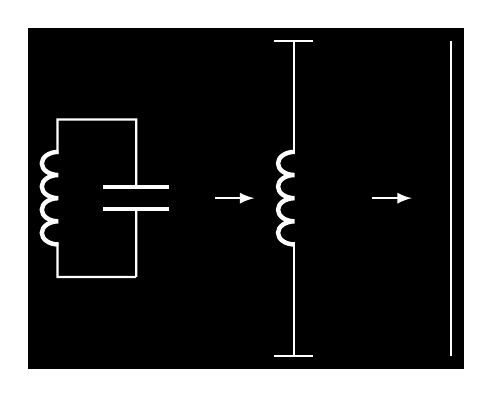
\begin{tikzpicture}[inverted,thick]
  \draw (0,0) to ++(-1,0) to[L] ++(0,2) to ++(1,0) to[C] ++(0,-2);
  %
  \draw[->] (1,1) to ++(0.5,0);
  %
  \draw (2,-1) to ++(0,1) to[L] ++(0,2) to ++(0,1);
  \draw (1.75,-1) to ++(0.5,0);
  \draw (1.75,3) to ++(0.5,0);
  %
  \draw[->] (3,1) to ++(0.5,0);
  %
  \draw (4,-1) to ++(0,4);
\end{tikzpicture}
\end{document}
